%% DCPAM —— 中文初稿（IEEE TIM 目标期刊，双栏 IEEEtran）
%% 编译：XeLaTeX（TinyTeX），建议 latexmk -xelatex main.tex
%% 说明：本文件为中文初稿，用于内容与逻辑打磨；后续将翻译为英文并套用最终期刊模板。
%%       未定的实验数值统一以「[待补：…]」占位，切勿视为真实结果。

\documentclass[journal]{IEEEtran}

% --- 中文支持（XeLaTeX + ctex）---
\usepackage{ctex}

% --- 常用宏包 ---
\usepackage{amsmath,amsfonts,amssymb}
\usepackage{bm}
\usepackage{graphicx}
\usepackage{array}
\usepackage{booktabs}
\usepackage{url}
\usepackage{cite}

% 图片搜索路径：直接复用 docs/ 下的原理图
\graphicspath{{figures/}{../docs/}}

% 占位命令：初稿中所有待补数值/内容用 \todo{...} 高亮标注
\newcommand{\todo}[1]{{\bfseries[待补：#1]}}

\begin{document}

\title{DCPAM：基于双相机与激光基准线的\\
点到轴距离测量模型}

\author{\todo{作者列表与单位}
\thanks{本文面向大型转动设备轴系对中的高精度非接触测量。}%
\thanks{稿件日期：\todo{投稿日期}。}}

\markboth{IEEE Transactions on Instrumentation and Measurement（中文初稿）}%
{DCPAM：基于双相机与激光基准线的点到轴距离测量模型}

\maketitle

\begin{abstract}
大型转动设备（汽轮机、发电机、压缩机等）的轴系对中精度直接决定机组的运行
平稳性与使用寿命。以火电厂汽轮机为例，转子直径通常在 1--2\,m 之间，对中精度
要求达到两丝（$20\,\mu\mathrm{m}$）量级。目前行业主流的钢丝找中法需要在待对中
轴之间反复拆装张紧的钢丝，不仅频繁干扰现场其他施工、在场地内构成绊拌等安全
隐患，钢丝自重引起的下坠挠度还会带来系统性的测量偏差。本文提出 DCPAM
（Dual-Camera-Based Point-to-Axis Measurement），用一条激光基准线替代钢丝，
通过前、后两个相机模块拍摄激光在毛玻璃接收屏上形成的光斑，经反投影、位姿对齐、
镜面虚像重建与点到直线距离计算，在统一的设备坐标系下恢复激光基准轴的三维空间
直线，并求解任意目标点到该轴的垂直距离。与只能读取激光斑在自身探测器上位置的
位置敏感探测器、需要合作反射器的激光跟踪仪，以及精度停留在毫米级的学术双目
激光线重建方法相比，DCPAM 直接面向“空间任意目标点到激光基准轴垂距”这一测量量，
目标精度为 $\pm15$--$50\,\mu\mathrm{m}$。实验部分给出重复精度评估与误差传播分析，
结果表明\todo{重复精度与主导误差来源结论}。

\end{abstract}

\begin{IEEEkeywords}
轴系对中，激光基准线，双目视觉，PnP 位姿估计，点到直线距离，镜面反射，精度分析。
\end{IEEEkeywords}

\section{概述}
\label{sec:intro}

大型转动设备是电力、船舶、航空等领域的核心动力装备。以火电厂
为例，汽轮机、发电机、给水泵等设备往往由多段转子串联组成一条长轴系，各段转子
之间通过联轴器连接。若相邻两段轴线之间存在偏移或折角，机组在运行时便会产生附加
的交变应力与振动，轻则加速轴承与密封件磨损，重则引发动静碰摩甚至断轴事故。因此，
轴系对中是设备安装与检修中的一道关键工序：需要精确测量待对中轴上若干采样点相对
某条理想基准轴的位置偏差，并据此调整设备的抬升与平移。汽轮机转子的直径通常在
1--2\,m 之间，工程上对相邻轴段的对中精度要求达到两丝，即 $20\,\mu\mathrm{m}$
量级，这对测量方法的分辨力与稳定性都提出了很高的要求。

目前行业内仍以钢丝找中法为主。其做法是在待对中的轴系中间张紧一根钢丝作为直线
基准，再用百分表或电接触方式逐点测量轴表面到钢丝的距离，从而还原各采样点相对
基准的偏差。这一方法原理直观、器材简单，但在现场使用中暴露出若干难以回避的缺陷。
其一，钢丝基准无法长期保留：每完成一轮测量都要拆除，隔日复测或调整之后复核时又
需重新架设与张紧，频繁的拆装既拖慢工期，也会干扰同一现场其他工序的并行施工。
其二，横贯现场的张紧钢丝处于人员通行的空间高度，容易绊拌施工人员，构成安全隐患。
其三，也是对精度影响最本质的一点，钢丝在自重作用下会产生下坠挠度，其垂度沿跨度
呈非线性分布并随张力波动，还对气流与机械振动敏感，使这条“基准直线”本身并不真正
是一条直线，从而在毫米量级引入难以彻底修正的系统偏差。

用一条激光束替代钢丝，是消除下坠挠度、免除反复拆装的自然思路。然而问题的难点并
不在于产生一条激光，而在于如何精确测量“空间中任意目标点到这条激光基准轴的垂直
距离”。判断一个已有方法是否可用，关键只看它能否（直接或间接）给出这一几何量，
而与其内部是否用到激光、激光扮演何种角色无关。以此为准，现有可比方案各有硬伤：
精度极高的激光跟踪仪须逐点安放合作反射器、成本高且效率低~\cite{api_radian,leica_at960}；
现役的位置敏感探测器靶板对中仪只能测激光斑击中探测器的那一单点~\cite{easylaser_xt770,fixturlaser_nxa}；
学术上最接近的双目激光线重建方法虽语义一致，精度却仅停留在毫米级~\cite{zhong2021line3d}。
这些方法与本文场景的具体差异将在第~\ref{sec:related} 节详细讨论。

针对上述空白，本文提出 DCPAM（Dual-Camera-Based Point-to-Axis Measurement）
测量模型。其核心思想是：用一条激光束充当替代钢丝的直线基准，在激光光路的前、后
两处各布置一个相机模块，每个模块通过一片 $45^\circ$ 倾斜的反射镜把激光引向一块
毛玻璃接收屏，相机隔着取景框拍摄激光在毛玻璃上漫散射形成的光斑。由两个模块拍到
的光斑分别反投影、并借助各自取景框的位姿标定统一到设备坐标系，再关于反射镜做
镜面反射得到激光的两个虚像点；这两个虚像点确定了激光基准轴在设备坐标系下的三维
空间直线，进而可对固定在测杆末端的目标点解析地计算其到该直线的垂直距离。整个
测量以非接触方式完成，激光基准不存在下坠问题，也无需在每次测量时重新架设。

本文的主要贡献可归纳为三点。首先，明确提出并形式化了“空间任意点到激光基准轴
垂距”这一在现有商业产品与文献中尚未被直接解决的测量问题，并系统梳理了相关方法
在该问题上的适用边界。其次，建立了基于双相机、接收屏与镜面虚像重建的完整几何
测量模型，给出从像素光斑到点线距离的端到端计算链路与相应的标定方法。最后，围绕
重复精度与误差传播开展了实验与精度分析，定位了当前系统的主导误差来源并指出
改进方向。本文其余部分组织如下：第~\ref{sec:related} 节梳理相关测量方法并定位
本文的空白；第~\ref{sec:model} 节给出 DCPAM 的坐标系约定、测量模型与标定方法；
第~\ref{sec:exp} 节报告实验结果与误差分析；第~\ref{sec:conclusion} 节总结全文
并展望后续工作。

\section{背景与相关工作}
\label{sec:related}

本节先对所要求解的测量量作形式化定义，并据此确立筛选相关方法的判据；随后依次讨论
在该判据下真正可比的方法及其局限，最后定位本文所填补的空白。

\subsection{问题定义与筛选判据}

给定空间中一条由激光定义的三维直线（激光基准轴 $\mathcal{L}$）与一个目标点
$P_T$，所要求解的物理量是 $P_T$ 到 $\mathcal{L}$ 的垂直距离 $H$。在大型转动设备
对中场景中，$\mathcal{L}$ 对应替代钢丝的理想基准轴，$P_T$ 对应待对中轴上的采样
点，$H$ 即该点相对基准的偏差。典型的精度需求为 $\pm15\,\mu\mathrm{m}$（理想）
到 $\pm50\,\mu\mathrm{m}$（工程可接受），量程为数米到数十米。

判断一个已有方法是否与本文相关，标准只有一个：它能否（直接或间接）给出“基准轴外
一点到该基准轴的距离”这一几何量。至于方法内部是否用到激光、其激光扮演什么角色，
与本判据无关——我们关心的是测量方法本身能否迁移到本文场景，而非其实现细节。据此，
一大类看似涉及“激光”的仪器其实并不可比：激光三角测距测的是传感器本体到目标表面
沿其光轴的单点位移，激光干涉测长测的是随动光学部件相对光路的位移，自准直仪测的
则是反射镜的角度。它们的输出量都不是“点到某条外部基准轴的距离”，也无法在不引入
额外基准定义的情况下迁移到本场景，因此不在本文的对比范围之内。下面只讨论在上述
判据下确实能测 $H$（或其变体）的方法，如表~\ref{tab:compare} 所示。

\begin{table*}[!t]
\centering
\caption{可测“点到基准轴距离”的方法对比}
\label{tab:compare}
\begin{tabular}{@{}p{2.6cm}p{3.0cm}p{2.4cm}p{4.2cm}@{}}
\toprule
方法 & 代表产品／文献 & 测 $H$ 的方式 & 主要局限 \\
\midrule
钢丝找中法 & 传统工装~\cite{wire_alignment} &
直接 & 钢丝下坠、振动敏感、需反复拆装、量程受限 \\
激光跟踪仪 & API Radian、Leica AT960~\cite{api_radian,leica_at960} &
间接（测坐标再算距离） & 需合作反射器，无法测非合作点，单价高 \\
双目激光线重建 & Zhong~\cite{zhong2021line3d}、Xu／Chen~\cite{xu2017ortho,chen2021vision2cam} &
直接（重建线／点） & 精度仅毫米级，达不到工程要求 \\
PSD／靶板对中仪 & Easy-Laser XT770、Fixturlaser NXA Pro~\cite{easylaser_xt770,fixturlaser_nxa} &
仅限受测单点 & 只能测激光斑击中探测器的那一点，换点须移装 \\
\textbf{DCPAM（本文）} & 双相机 + 接收屏 + 镜面虚像重建 &
\textbf{直接（对任意点）} & 依赖 PnP 与镜面装配标定精度 \\
\bottomrule
\end{tabular}
\end{table*}

\subsection{传统钢丝找中法}

在所有方法中，唯一与 $H$ 语义完全一致、且现场长期沿用的是传统钢丝找中法~\cite{wire_alignment}。
它以一根张紧钢丝作基准直线，逐点测量轴表面到钢丝的垂直距离，测的正是“点到基准轴
距离”，因而是本文最直接的对标对象，也是要替代的方法。其局限已在第~\ref{sec:intro}
节详述：钢丝自重下坠使基准并非真正的直线、对气流与振动敏感、且每轮测量都需反复
架设拆装。DCPAM 保留了“点到基准轴距离”这一测量语义，同时用激光基准消除下坠、
用非接触方式免除反复拆装。

\subsection{激光跟踪仪与全站仪}

激光跟踪仪用角度编码器加测距单元跟踪一个合作反射器（SMR），输出反射器球心的三维
坐标，代表产品如 API Radian~\cite{api_radian} 与 Leica Absolute Tracker
AT960~\cite{leica_at960}，其三维定位精度往往优于本文目标，量程也大得多。它可以
间接得到 $H$：先用反射器在基准轴上取两点拟合出轴线、再逐点巡测目标并按叉积公式
计算点到轴距离。就“能否测 $H$”而言，它是可行且精度很高的方案。真正的障碍在于
适用性：所有目标点都必须能够安放合作反射器，跟踪仪无法直接测量非合作的空间特征
点；逐点巡测需要人工把反射器依次移动到每个采样点，效率低；且设备单价高昂，难以
在现场大批量采样点的对中作业中普遍配备。因此它在实验室级少点位测量中可用，却不
适配本文面向的现场高密度对中场景。

\subsection{双目与多目立体视觉激光线重建}

学术上与本文思路最接近的是用立体视觉重建激光相关几何量的工作，也是需要重点区分
的方向。Zhong 等提出的线性三维直线重建方法先由对应点交会求线上一点、再最小化
图像角度残差求线方向，可用于双目与多目重建~\cite{zhong2021line3d}，重建出三维
直线后即可对任意点算叉积距离，与本文测量语义直接一致；但其在 30\,cm 长目标上的
距离误差为毫米量级，与本文 $15$--$50\,\mu\mathrm{m}$ 的目标相差一到两个数量级。
另有一类以正交参考物或三维定向参考物辅助双相机重建的工作，如 Xu 等借助正交参考
重建激光线投影点~\cite{xu2017ortho}、Chen 等用双相机配合三维定向参考做视觉重建
与精度分析~\cite{chen2021vision2cam}，其绝对误差约 $1\,\mathrm{mm}$。这一类方法
在“重建激光相关的三维几何量、进而可算距离”这一点上与本文可比，其共同短板是精度
停留在毫米级，无法满足工程要求。DCPAM 与之的核心区别有三：其一，采用接收屏配合
镜面反射虚像重建，把激光基准轴变为设备坐标系下可解析的三维直线，回避了从三维
空间中直接提取“看不见的激光”这一难题；其二，直接面向“任意目标点到基准轴距离”
求解，无需额外的外部参考物建立尺度；其三，精度目标比上述方法高出一到两个数量级。

\subsection{位置敏感探测器与靶板式对中仪}

工业界最主流的商用激光对中仪采用位置敏感探测器（PSD）或 CCD/CMOS 靶板：在一根轴
上安装激光发射器、在另一根轴上安装探测器，读取激光斑落在感光面上的坐标，再结合
轴的多角度旋转数据反算两轴之间的偏移与折角，代表产品如 Easy-Laser
XT770~\cite{easylaser_xt770}、Fixturlaser NXA Pro~\cite{fixturlaser_nxa} 与
Pr\"uftechnik Optalign Touch~\cite{pruftechnik_optalign}。就测量语义而言，它测的
确实是“某一点相对激光的位置”，但这一点只能是激光斑恰好击中的探测器所在位置：单点
探测分辨力虽可达微米级，却只覆盖被测的那一个点，要测另一个目标点就必须把探测器
物理搬到该点重装，无法对不在光路上、也不便安装传感器的采样点做非接触测量。因此
它虽是现役竞品，却只能逐点接触式测量、且输出的最终量是两轴的相对偏移与角度，难以
胜任对空间任意点求 $H$ 的任务。

\subsection{空白定位}

综合来看，如表~\ref{tab:compare} 所示，在“对空间任意目标点求点到激光基准轴距离”
这一测量量上，现有方案各有硬伤：语义完全匹配的钢丝找中法受下坠、振动与反复拆装
限制；精度极高的激光跟踪仪必须逐点安放合作反射器、成本高且效率低；语义直接一致的
学术双目激光线重建精度只到毫米级；现役的 PSD 靶板对中仪则只能测激光斑击中的那一
单点。真正能对空间任意点、以非接触方式、达到微米级精度地直接求 $H$ 的方法尚属
空白。DCPAM 正是要填补这一空白——用双相机加接收屏镜面虚像重建，把激光基准轴变为
设备坐标系下可解析的三维直线，从而对空间任意目标点直接解析地计算 $H$。

\section{测量模型与建模}
\label{sec:model}

本节给出 DCPAM 的完整建模过程：先约定坐标系与关键符号，再给出总测量模型，
随后逐步展开从像素光斑到点线距离的四步计算链路，最后说明所依赖的标定方法，
并把整条链路整理为便于误差分析的端到端仿射形式。

\subsection{坐标系约定}

系统涉及三个坐标系。前相机坐标系记为 $C_1$，后相机坐标系记为 $C_2$，二者的
原点分别位于对应相机光心，$Z$ 轴沿各自光轴指向物方，均为右手系；相机光心在
自身坐标系中恒为 $(0,0,0)^\mathsf{T}$，这是坐标系定义，不由内参计算得到。设备
坐标系记为 $D$，是算法的主坐标系，定义为前取景框的局部系：原点取前取景框中心，
$+X$ 由前相机模块指向后相机模块，$+Y$ 沿画面自上而下，$+Z$ 指向远离相机的
方向（即毛玻璃一侧），亦为右手系。前、后两个模块拍到的实像点最终都统一到 $D$ 下
完成镜面反射、激光线构造与距离计算；两相机之间的外参不参与主链路，坐标统一改由
各模块取景框的位姿标定完成，具体见第~\ref{subsec:calib} 节。

这里需要区分两个易混概念。设备上的物理基准面称为“设备实像面”，即毛玻璃紧贴
取景框、位于设备坐标系 $Z=0$ 的那一面；而“PnP 实像面”是由取景框位姿标定得到的、
位于相机坐标系下的实像面估计。建模的核心工作之一，就是把 PnP 实像面与设备坐标系
中的设备实像面对齐，从而把相机系下的量搬入设备系。

\subsection{总测量模型}

DCPAM 的输入是前、后相机采集的两幅图像与测杆工装长度，输出是目标点到激光基准轴
的距离，整体模型可写为
\begin{equation}
\label{eq:dcpam}
h_t = \mathrm{DCPAM}(I_{C_1},\, I_{C_2},\, l_T),
\end{equation}
其中 $I_{C_1}$、$I_{C_2}$ 分别为相机 $C_1$、$C_2$ 采集的图像，$l_T$ 为测杆工装
长度，$h_t$ 为目标点到激光基准线的垂直距离。表~\ref{tab:symbols} 列出建模过程中
用到的关键点符号及其所属坐标系。

\begin{table}[t]
\centering
\caption{关键坐标点符号}
\label{tab:symbols}
\begin{tabular}{@{}llp{3.6cm}@{}}
\toprule
符号 & 坐标系 & 含义 \\
\midrule
$P^f_{\mathrm{real}}$      & $D$   & 前接收屏上的激光实像点（并入设备系后） \\
$P^b_{\mathrm{real}}$      & $D$   & 后接收屏上的激光实像点（并入设备系后） \\
$P^f_{\mathrm{virtual}}$   & $D$   & 前反射镜镜像得到的激光虚像点 \\
$P^b_{\mathrm{virtual}}$   & $D$   & 后反射镜镜像得到的激光虚像点 \\
$P_T$                      & $D$   & 目标点（测杆末端靶点） \\
\bottomrule
\end{tabular}
\end{table}

模型的几何直觉是：激光被前、后两片倾斜反射镜分别折向各自的毛玻璃接收屏，
相机拍到的是激光在接收屏上的实像；把这两个实像点关于各自反射镜做镜面反射，即可
在设备坐标系下还原出激光被折射之前所在的两点，这两个虚像点确定了激光基准轴的
空间直线，目标点到该直线的垂距即为所求。

\subsection{四步计算链路}

DCPAM-CV 的计算链路可分为四步。之所以这样划分，是因为前三步各自对应一个相互
独立的误差来源：第一步的光斑圆心提取取决于像素定位精度，第二步的反投影与转入
取景框局部系取决于 PnP 定位精度，第三步的统一到设备坐标系与镜面反射取决于设备
几何尺寸的测量与安装精度；三者互不影响。第四步只是最终的距离结算，本身不引入新
的误差，其误差完全由前三步传递而来。这一划分与第~\ref{sec:exp} 节的误差分析
一一对应。

\subsubsection{光斑提取}
首先从前、后相机图像中提取激光光斑的圆心像素坐标 $(u_1,v_1)$ 与 $(u_2,v_2)$，
写成齐次形式
\begin{equation}
\label{eq:pixel}
\bm{p}_1 = (u_1, v_1, 1)^\mathsf{T}, \qquad
\bm{p}_2 = (u_2, v_2, 1)^\mathsf{T}.
\end{equation}
激光打在毛玻璃上形成的光斑较大且中心饱和，圆心定位的稳健性对最终精度影响显著，
相关分析见第~\ref{sec:exp} 节。

\subsubsection{反投影与位姿对齐}
本步取决于 PnP 定位精度。已知相机内参矩阵
$K$，先把像素点去畸变后反投影为相机坐标系下的一条视线方向
$\bm{r}=\mathrm{undistort}(K^{-1}\bm{p})$，再令该视线与相机系下的成像面求交。
若成像面方程为 $\bm{n}^\mathsf{T}\bm{x}+d=0$，视线为 $\bm{x}=\lambda\bm{r}$，则
交点参数与相机系下的实像点为
\begin{equation}
\label{eq:intersect}
\lambda = -\frac{d}{\bm{n}^\mathsf{T}\bm{r}}, \qquad
P_{\mathrm{real}}^{\text{cam}} = \lambda\bm{r}.
\end{equation}
再由 PnP 标定得到的相机到取景框局部系的刚体位姿，把实像点从相机系转入各自取景框
局部系：前相机点经 $T_{C_1\to\text{frame}_f}$ 转入前框局部系，后相机点经
$T_{C_2\to\text{frame}_b}$ 转入后框局部系。反投影与位姿对齐共用同一套 PnP 标定
结果，误差同源。

\subsubsection{坐标统一与镜面重建}
本步取决于设备几何尺寸的测量与安装精度。前取景框局部系即取为设备系 $D$，故前框
实像点已在设备系中；后框实像点再经后框到前框的 6DOF 装配变换 $T_{b\to f}$ 并入
设备系：
\begin{equation}
\label{eq:to_device}
P^f_{\mathrm{real}} = P^{f,\text{frame}_f}_{\mathrm{real}}, \qquad
P^b_{\mathrm{real}} = T_{b\to f}\, P^{b,\text{frame}_b}_{\mathrm{real}}.
\end{equation}
随后在设备坐标系下，把两个实像点分别关于对应反射面做镜面反射，还原激光被折射前
的位置。若反射面方程为 $\bm{n}^\mathsf{T}\bm{x}+d=0$，则点 $\bm{x}$ 的镜像点为
\begin{equation}
\label{eq:mirror}
\bm{x}_{\mathrm{mirror}} = \bm{x} - 2(\bm{n}^\mathsf{T}\bm{x}+d)\,\bm{n},
\end{equation}
于是
\begin{equation}
\label{eq:virtual}
\begin{aligned}
P^f_{\mathrm{virtual}} &= \mathrm{mirror}(P^f_{\mathrm{real}}, M_f), \\
P^b_{\mathrm{virtual}} &= \mathrm{mirror}(P^b_{\mathrm{real}}, M_b),
\end{aligned}
\end{equation}
其中 $M_f$、$M_b$ 为设备系下的前、后反射面。反射镜两面平行度极高，建模时用单面
近似，忽略镜片厚度带来的折射偏置。装配变换与反射面同为设备几何量，误差同源。

\subsubsection{点线距离结算}
本步是最终的距离结算，仅由前三步的输出解析地算得，本身不引入独立误差，其误差
完全由前三步传递而来。前、后两个虚像点确定了激光基准轴的空间直线。记方向向量
$\bm{L}=P^f_{\mathrm{virtual}}-P^b_{\mathrm{virtual}}$ 与
$\bm{w}=P_T-P^b_{\mathrm{virtual}}$，目标点 $P_T$ 到该直线的垂直距离由叉积公式
给出：
\begin{equation}
\label{eq:distance}
H = \frac{\lVert \bm{L}\times\bm{w}\rVert}{\lVert \bm{L}\rVert}.
\end{equation}
目标点由设备几何中的测杆直接给定，$P_T=(x_0,y_0,z_0-l_T)^\mathsf{T}$，其中
$(x_0,y_0,z_0)$ 为杆根安装位置，$l_T$ 为测杆长度、靶点沿 $Z$ 负向延伸。
图~\ref{fig:principle} 给出上述链路的几何示意。

\begin{figure}[t]
\centering
% 优先复用 docs/原理图.png；若清晰度不足需重画，见 \todo
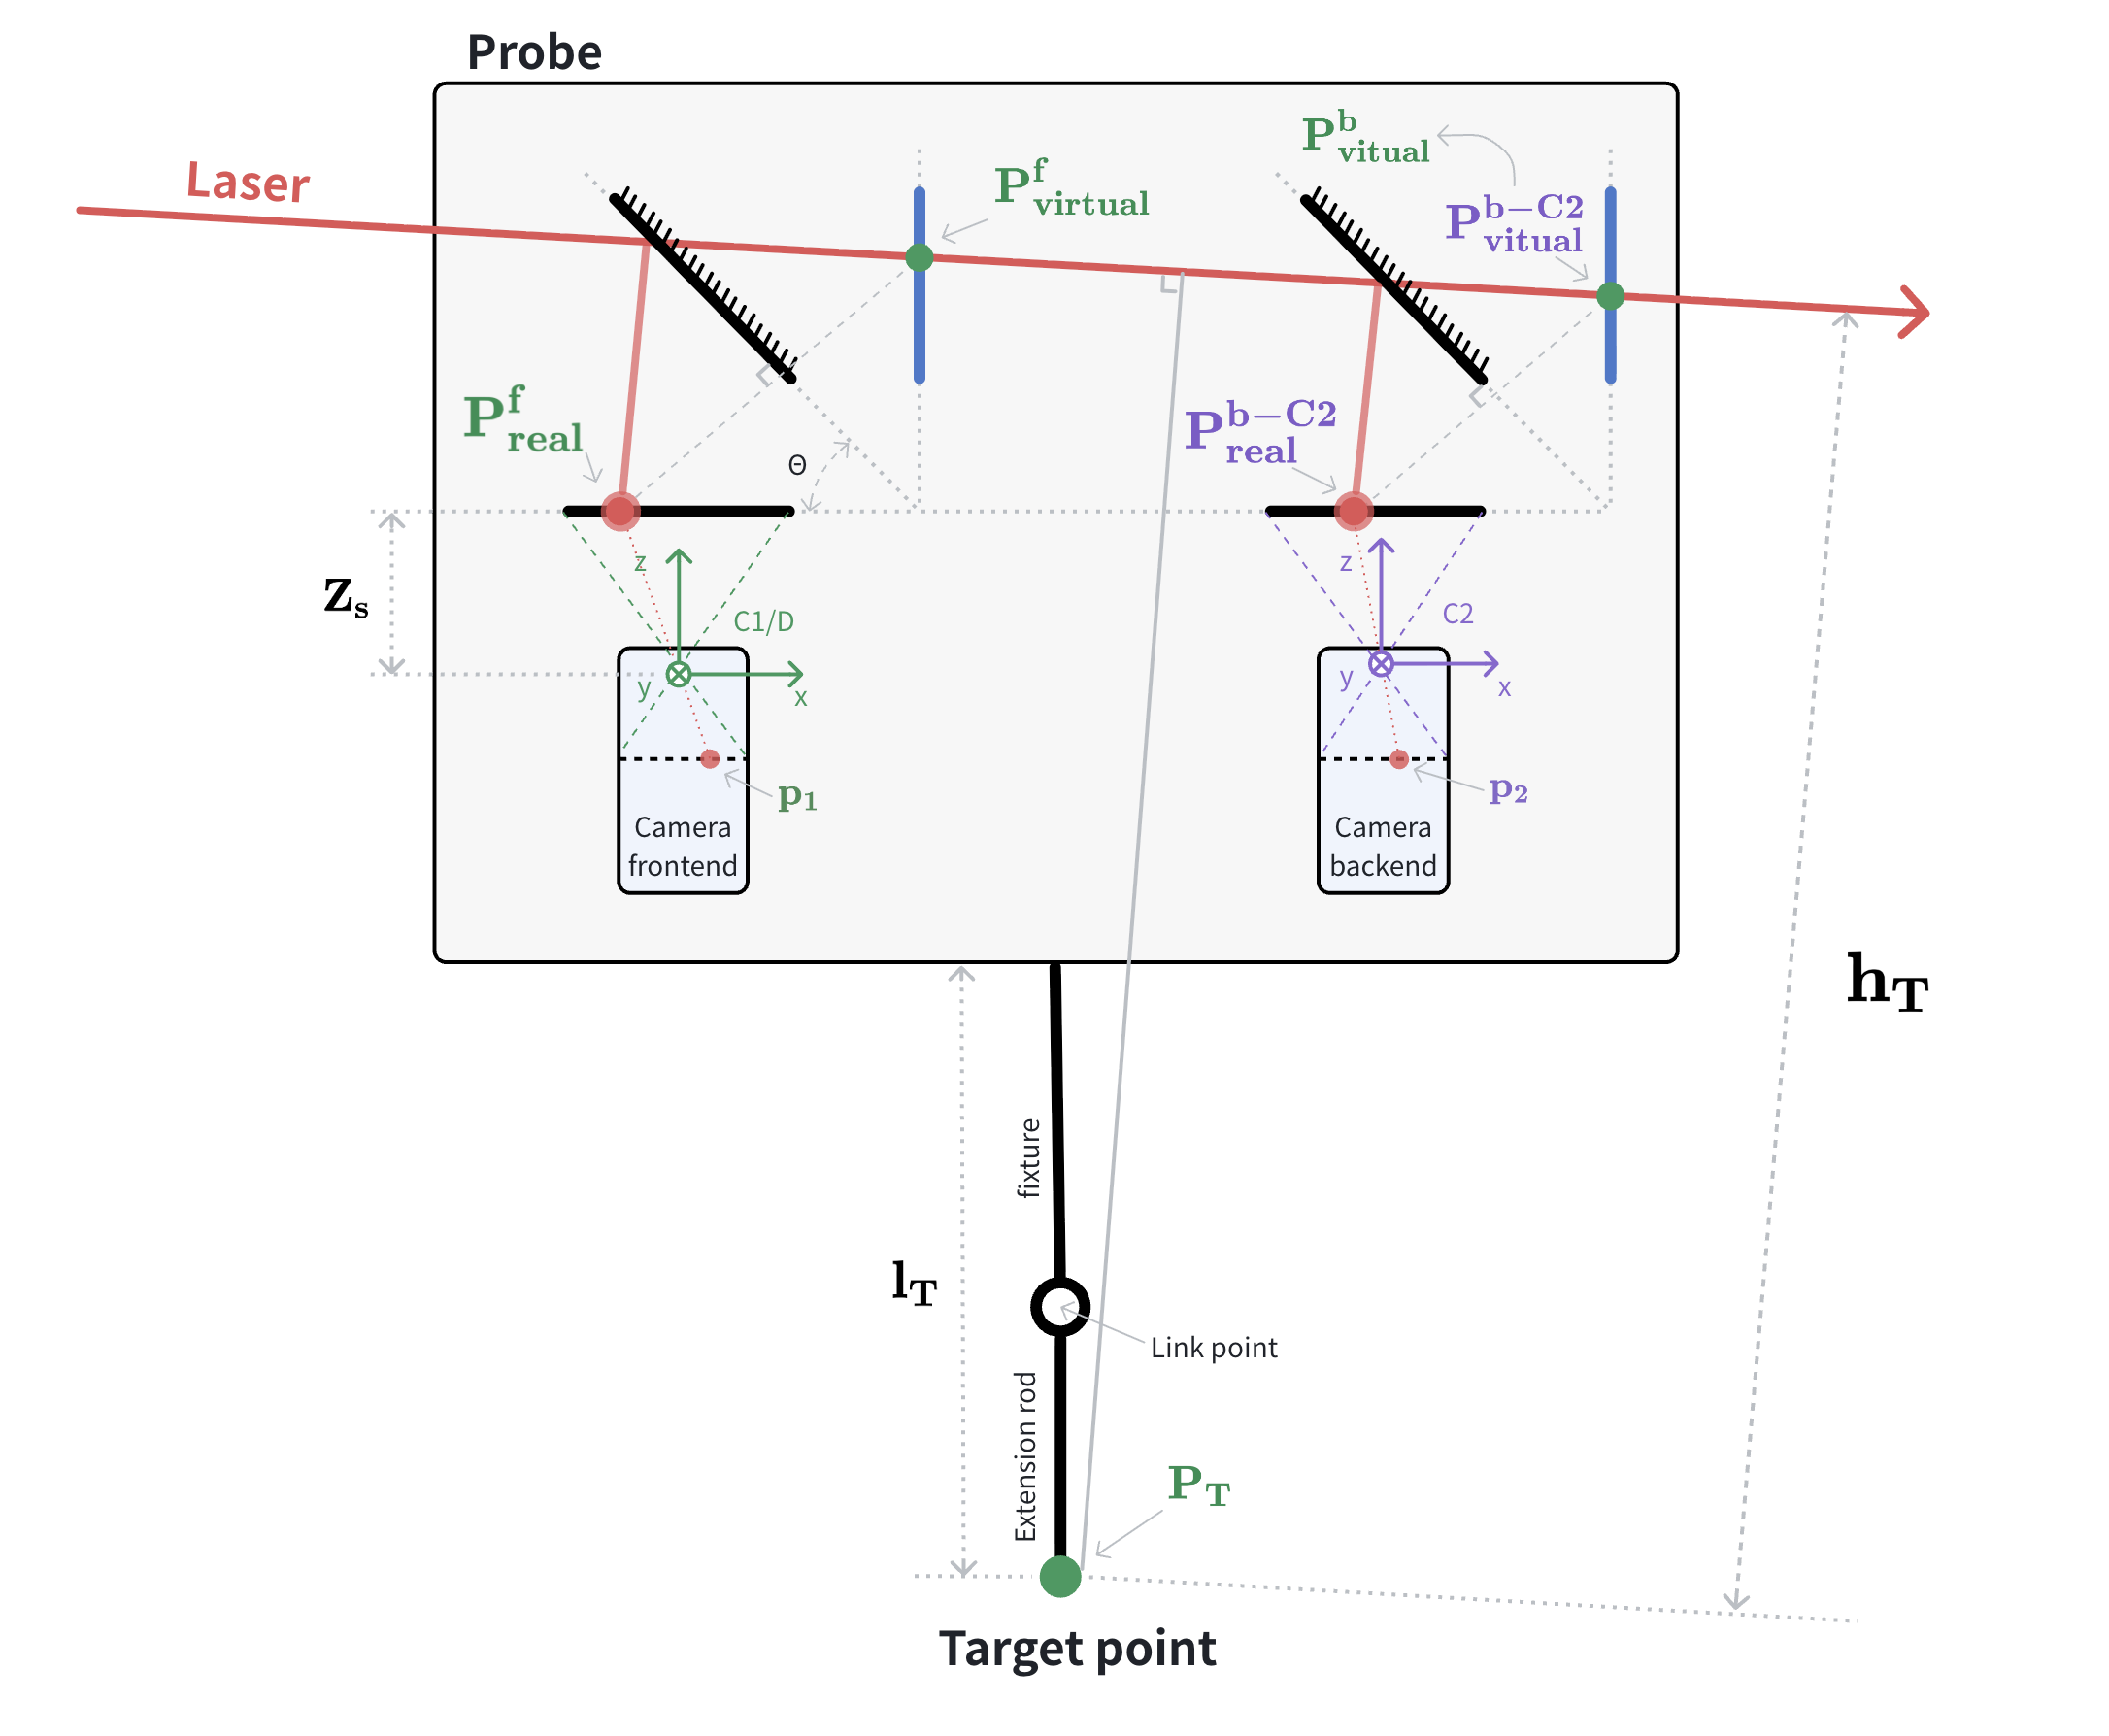
\includegraphics[width=\columnwidth]{原理图.png}
\caption{DCPAM 测量原理示意：激光经前后倾斜反射镜折向各自毛玻璃接收屏，
相机拍摄光斑实像，经镜面反射还原为设备坐标系下的虚像点，确定激光基准轴并计算
目标点垂距。\todo{按最终版式重绘为矢量图并统一符号}}
\label{fig:principle}
\end{figure}

\subsection{标定}
\label{subsec:calib}

模型依赖三类标定。第一类是相机内参：采用 OpenCV 针孔模型，标定焦距
$f_x,f_y$、主点 $(c_x,c_y)$ 与畸变系数 $k_1,k_2,p_1,p_2$，构成内参矩阵
$K=\left[\begin{smallmatrix} f_x&0&c_x\\ 0&f_y&c_y\\ 0&0&1\end{smallmatrix}\right]$，
用于式~\eqref{eq:intersect} 的反投影。第二类是相机与取景框之间的位姿，采用五
圆点 PnP 定位法：每个取景成像面上贴五个黑色圆点，其在成像面局部系下的三维坐标
由影像仪测出作为物点，标定时从相机图像中提取五个圆心像素与物点做 PnP，解出相机
到取景框局部系的刚体位姿，即式~\eqref{eq:intersect} 之后转入局部系所需
的 $T_{C_1\to\text{frame}_f}$ 与 $T_{C_2\to\text{frame}_b}$，同时得到相机系下的成像面平面。
第三类是设备几何，包括设备系下的前、后反射面、后框到前框的装配变换 $T_{b\to f}$
以及测杆的杆根位置与长度，由人工测量结合影像仪与
关节臂实测确定。需要说明的是，历史上曾用双相机外参做坐标统一，但微距镜头下两相机
无法对同一成像面合焦、外参可靠性不足，因此主链路改用上述以设备坐标系为中心的
标定方案，不再依赖双相机外参。

\subsection{端到端仿射形式}

把式~\eqref{eq:pixel}--\eqref{eq:virtual} 的反投影、坐标统一与镜面反射整条链路
组合起来，在局部小扰动范围内，每个虚像点的坐标都是对应像素坐标的仿射函数：
\begin{equation}
\label{eq:affine_f}
\begin{aligned}
x_f &= A_1 u_1 + B_1 v_1 + C_1, \\
y_f &= D_1 u_1 + E_1 v_1 + F_1, \\
z_f &= G_1 u_1 + H_1 v_1 + I_1,
\end{aligned}
\end{equation}
后虚像点 $(x_b,y_b,z_b)$ 关于 $(u_2,v_2)$ 有同样形式，系数 $A_1,\dots,I_2$ 由
复合矩阵乘积确定。据此可得一个对精度分析很有用的结论：距离 $H$ 的绝对值随测杆
长度 $l_T$ 改变，但当 $l_T$ 固定时，由像素提取噪声引起的距离变化量 $\Delta H$
几乎不依赖 $l_T$，仅由像素噪声与系统系数决定。这一线性化关系是第~\ref{sec:exp}
节误差传播与灵敏度分析的基础。

\section{实验与精度分析}
\label{sec:exp}

本节围绕三条主线展开：一是验证系统的重复精度（同一位置多次测量的一致性）是否
达标，二是通过独立高精度参考验证测量的绝对准确度，三是分析测量精度受哪些因素
影响并定位主导误差来源。需要说明的是，本节部分定量结果仍在补充实验中，相应数值
以占位形式标注，不作为最终结论。

\subsection{实验装置与数据采集}

样机由前、后两个相机模块沿设备 $X$ 方向并排组成，两模块中心间距约
$80\,\mathrm{mm}$。每个模块含一片 $45^\circ$ 反射镜（实测夹角 $45.22^\circ$、
厚约 $1.05\,\mathrm{mm}$、两面平行度优于 $0.06^\circ$）与一块紧贴取景框的毛
玻璃接收屏（取景框与毛玻璃叠层总厚约 $5\,\mathrm{mm}$）。相机分辨率为
$2592\times1944$。测杆固定在底板上方，靶点位于杆末端。设备各面的绝对位置与
反射镜、测杆的几何参数由影像仪与关节臂配合标定，作为设备坐标系几何真值的对照
基准。采集时对同一目标位置连续突发拍摄 $N$ 帧、取圆心均值以抑制随机噪声，并
按“杆长—距离”分组多次重复，用于统计重复精度。真值参考由关节臂扫描给出。

\subsection{重复精度}

重复精度以每组重复测量的组内标准差 $\hat{\sigma}_H$ 衡量。当前基线下，全体
测量组的平均组内标准差约为 \todo{重复精度 $\hat{\sigma}_H$ 终值}，与工程目标
$\pm15$--$50\,\mu\mathrm{m}$ 之间的关系为 \todo{是否达标的结论}。在优化过程中
发现，圆心提取策略对重复精度具有决定性影响：激光光斑并非小圆点，而是半径约
$120\,\mathrm{px}$、中心大面积饱和且带有不对称暗弱拖尾的大斑；早期采用的小
窗口、低阈值强度加权重心会把拖尾纳入重心而被拉偏，改为覆盖整斑的大窗口配合高
阈值后，平均组内标准差从约 $216\,\mu\mathrm{m}$ 降至约 $106\,\mu\mathrm{m}$，
接近腰斩。这一改进已合入测量流程。相关分组重复精度的完整统计见
表~\ref{tab:repeat}。

\begin{table}[t]
\centering
\caption{分组重复精度统计（组内标准差 $\hat{\sigma}_H$）}
\label{tab:repeat}
\begin{tabular}{@{}lccc@{}}
\toprule
分组（杆长／距离） & 重复次数 & $\hat{\sigma}_H/\mu\mathrm{m}$ & 备注 \\
\midrule
\todo{组1} & \todo{$n$} & \todo{$\sigma$} & \\
\todo{组2} & \todo{$n$} & \todo{$\sigma$} & \\
平均       & --          & \todo{均值}     & \\
\bottomrule
\end{tabular}
\end{table}

\subsection{绝对值验证}

重复精度只反映同一位置多次测量的一致性，即测量的稳定性，却不能说明测得的距离
是否接近真值——一个系统可能重复性很好却存在稳定的系统偏差。因此还需对测量的
绝对准确度单独验证。由于“空间任意点到激光基准轴距离”这一测量量此前尚无成熟的
标准量具或公认的参考方法，我们无法直接购置一台已校准的仪器作真值来源，只能自行
搭建一套独立的高精度参考实验。

我们计划在实验室环境下借助激光跟踪仪构建参考基准。如第~\ref{sec:related} 节所
分析，激光跟踪仪的三维定位精度显著优于本文目标，虽因需逐点安放合作反射器而不适
用于现场高密度对中，却恰好适合在实验室对少量标定点提供独立、可溯源的高精度坐标
参考。具体方案是：用激光跟踪仪配合合作反射器测量激光基准轴上若干点以独立拟合出
基准轴，再测量各目标点坐标并按点到直线公式算出参考距离 $H_{\mathrm{ref}}$；将
DCPAM 在同一批目标点上测得的 $H_{\mathrm{DCPAM}}$ 与 $H_{\mathrm{ref}}$ 逐点
比较，以偏差 $H_{\mathrm{DCPAM}}-H_{\mathrm{ref}}$ 的均值刻画系统性误差（trueness）、
以其标准差与重复精度相互印证，从而给出 DCPAM 的绝对准确度评估。

该实验尚在进行中，结果留待补充：绝对偏差均值为 \todo{系统偏差均值}，偏差标准差
为 \todo{偏差标准差}，与工程目标 $\pm15$--$50\,\mu\mathrm{m}$ 的关系为
\todo{绝对准确度是否达标的结论}。

\subsection{误差来源与灵敏度分析}

测量误差可归为测量端与几何端两类。测量端的主导来源是圆心提取的像素噪声：即便
在亚像素级（跨图圆心标准差约 $0.3$--$0.7\,\mathrm{px}$），其经由整条链路传播后
仍构成 $\hat{\sigma}_H$ 的主要成分。这一噪声进一步被光路几何放大——分析表明，
组内标准差与虚像点在 $Z$ 方向的离散强相关（相关系数约 $0.944$），像素扰动经
约 $740\,\mathrm{mm}$ 的杠杆臂放大后显著抬升了 $H$ 的波动，因此 $Z$ 方向的杠杆
敏感度是需要在光路与靶点几何设计上重点抑制的因素。此外，激光器自身的指向抖动、
相机在采集期的机械抖动，以及曝光不一致带来的采集期漂移，都会叠加到圆心的帧间
波动上，其量级需通过专门实验分别标定，此处以占位标注：激光抖动
\todo{激光抖动贡献}、相机抖动 \todo{相机抖动贡献}、PnP 定位精度
\todo{PnP 复现精度}。

几何端的敏感度则相对次要。围绕反射面平移与设备几何参数所做的偏移扫描与自标定
实验表明，当前设备几何已接近物理真值：把反射镜夹角、模块间距、装配旋转、测杆
杆根与杆长等参数放开做以组内方差为目标的自标定，各参数仍稳定落在物理真值附近
（如反射镜夹角约 $45^\circ$、模块间距约 $80\,\mathrm{mm}$、装配旋转小于
$0.01^\circ$），而平均组内标准差仅改善约 $5\%$。这从反面印证了两点：其一，
几何标定已到位、无需再调；其二，$\hat{\sigma}_H$ 的主导来源并非几何参数，而是
测量端的像素噪声。因此，降低方差的主战场在测量端而非几何参数。

\subsection{误差传播与蒙特卡洛验证}

基于第~\ref{sec:model} 节的端到端仿射形式，把 $H$ 对四个像素坐标的一阶泰勒
展开写为
\begin{equation}
\label{eq:propagation}
\sigma_H^2 \approx \sum_{q\in\{u_1,v_1,u_2,v_2\}}
\left(\frac{\partial H}{\partial q}\right)^2 \sigma_q^2,
\end{equation}
并定义各像素坐标的方差贡献占比
\begin{equation}
\label{eq:eta}
\eta_q = \frac{(\partial H/\partial q)^2\,\sigma_q^2}{\sigma_H^2}\times 100\%.
\end{equation}
为验证解析式，对每个像素坐标在 $\pm1\,\mu\mathrm{m}$ 范围内独立扰动做
$N=10^4$ 次蒙特卡洛采样，比较经验标准差 $\hat{\sigma}_H$ 与解析值 $\sigma_H$。
二者的一致性结果为 \todo{解析 $\sigma_H$ 与 MC $\hat{\sigma}_H$ 对照值}，
各像素坐标的灵敏度占比 $\eta_q$ 为 \todo{$\eta_q$ 分布}，与前述“$Z$ 向杠杆
放大像素噪声”的判断相互印证。

\subsection{讨论}

综合上述结果，当前系统的重复精度与 $\pm15$--$50\,\mu\mathrm{m}$ 的工程目标之间
\todo{差距量化}，其瓶颈明确位于测量端的像素噪声及其经 $Z$ 向杠杆的放大，而非
几何标定。据此，后续改进应从三方面着手：进一步提升圆心提取精度或改用更高信噪比
的相机与激光源，以直接压低像素噪声；通过光路与靶点几何设计降低 $Z$ 方向的杠杆
敏感度；以及改善采集条件（统一曝光、抑制采集期漂移与机械抖动）。这些方向所对应
的定量收益将在补充实验中给出。

\section{结论}
\label{sec:conclusion}

本文针对大型转动设备轴系对中中“空间任意点到激光基准轴垂直距离”这一在现有商业
产品与文献中尚未被直接解决的测量问题，提出了 DCPAM 测量模型。该模型以一条激光束
替代传统钢丝找中法中的张紧钢丝，消除了钢丝下坠挠度带来的系统偏差，并免除了每次
测量时反复架设钢丝所引发的工期干扰与安全隐患。方法上，通过前、后两个相机模块
拍摄激光在毛玻璃接收屏上的光斑，经反投影、基于五圆点 PnP 的位姿对齐、设备坐标系
下的镜面虚像重建与叉积点线距离计算，把激光基准轴还原为设备坐标系下可解析的三维
直线，从而对任意目标点直接求解其到该轴的垂距。

围绕重复精度与误差传播的实验与分析表明，系统的主导误差来源位于测量端的圆心提取
像素噪声，并经 $Z$ 方向的光路杠杆放大，而设备几何参数已接近物理真值、并非方差的
主要杠杆；改进圆心提取显著降低了重复测量的组内标准差。当前重复精度与
$\pm15$--$50\,\mu\mathrm{m}$ 工程目标之间的差距及其定量结论仍在补充实验中完善。

后续工作将从三方面推进。其一，在测量端进一步压低像素噪声，包括用卷积神经网络直接
从原始图像回归光斑圆心以替代部分手工特征提取，以及改用更高信噪比的相机与激光源。
其二，建立测杆倾斜偏差 $\beta$ 与测量精度的关系模型，给出在指定精度下的倾斜度
舍弃阈值，并通过光路与靶点几何设计降低 $Z$ 向杠杆敏感度。其三，完善全量关节臂
扫描标定与标定一致性自检，进一步巩固几何真值并支撑现场大批量采样点的对中作业。


\bibliographystyle{IEEEtran}
\bibliography{refs}

\end{document}
